\documentclass{article}


\usepackage{neurips_data_2024}


\usepackage[utf8]{inputenc} % allow utf-8 input
\usepackage[T1]{fontenc}    % use 8-bit T1 fonts
\usepackage{hyperref}       % hyperlinks
\usepackage{url}            % simple URL typesetting
\usepackage{booktabs}       % professional-quality tables
\usepackage{amsfonts}       % blackboard math symbols
\usepackage{nicefrac}       % compact symbols for 1/2, etc.
\usepackage{microtype}      % microtypography
\usepackage{xcolor}         % colors
\usepackage{graphicx} 

\title{Assignment 2: NBA Dataset}


\author{%
 Sean Mahlanza (2438634) \\ 
 Phemelo Masilo (2444482) \\
 Gael Joao (2494554) \\
 Blessing Kodze (2560370) \\
}

\begin{document}

\maketitle

\begin{abstract}
  The abstract paragraph should be indented \nicefrac{1}{2}~inch (3~picas) on
  both the left- and right-hand margins. Use 10~point type, with a vertical
  spacing (leading) of 11~points.  The word \textbf{Abstract} must be centered,
  bold, and in point size 12. Two line spaces precede the abstract. The abstract
  must be limited to one paragraph.
\end{abstract}

\section{Data Cleaning}

The NBA 2022-23 statistics dataset underwent systematic data cleaning and preprocessing to ensure data quality and prepare it for machine learning analysis. First, we removed the redundant index column (\texttt{Unnamed: 0}) that duplicated the DataFrame's built-in index. We then addressed data type inconsistencies, particularly in the \texttt{3P} (3-Point Field Goals Made) column, which contained string values with spurious 's' characters (e.g., '1.s6' instead of '1.6'). Missing values in shooting percentage columns (\texttt{3P\%}, \texttt{FT\%}, \texttt{FG\%}, etc.) were filled with zero, as these typically indicated zero attempts rather than missing data. To address data quality concerns related to players with minimal playing time, we applied minimal filtering criteria, retaining only players with at least 5 games played and 25 total minutes, which removed approximately 467 players with negligible statistical impact while preserving meaningful data. For machine learning applications, we removed identifier columns (\texttt{Player Name}, \texttt{Team}, \texttt{Position}), applied log transformation to the \texttt{Salary} feature to reduce skewness, split the data into training (70\%), validation (15\%), and test (15\%) sets with a fixed random seed (42) for reproducibility, and standardized all features to zero mean and unit variance using \texttt{StandardScaler}. This comprehensive preprocessing pipeline resulted in 48 numeric features ready for dimensionality reduction and clustering analysis.

\section{Dimensionality Reduction}

\subsection{Autoencoder Architecture and Training}

We implemented a deep autoencoder using PyTorch to learn a compressed 2-dimensional representation of the 48-dimensional NBA player statistics. The autoencoder consists of an encoder network that compresses the input through progressively smaller hidden layers [128, 96, 64, 32] to a 2-dimensional latent space (compression ratio of 24:1), and a symmetric decoder network that reconstructs the original features from the latent representation. The architecture uses ReLU activation functions for non-linearity and was trained using the Adam optimizer with a learning rate of $5 \times 10^{-5}$ and batch size of 16.

The training process employed early stopping with a patience of 30 epochs to prevent overfitting, monitoring validation loss on a held-out validation set (15\% of data). The model converged after 336 epochs with a best validation loss of 0.298 (MSE) and demonstrated good generalization (training/validation ratio of 1.075). The final model achieved a mean reconstruction error of 0.395 (MSE) on the test set, with an RMSE of 0.629, indicating that the 2D latent space successfully captures the essential structure of the 48-dimensional player statistics while discarding noise.

\subsubsection{K-Means Clustering on 2D Latent Space}

We applied k-Means clustering (k=5) directly to the 2D autoencoder latent representations to identify distinct player archetypes. This approach leverages the autoencoder's learned compressed representation to group players by statistical similarity. Table~\ref{tab:ae_cluster_stats} presents the statistical profiles of each cluster.

\begin{table}[h!]
\centering
\caption{Autoencoder K-Means Cluster Statistical Summary}
\label{tab:ae_cluster_stats}
\begin{tabular}{lcccccc}
\toprule
\textbf{Cluster} & \textbf{PTS} & \textbf{AST\%} & \textbf{STL\%} & \textbf{BLK\%} & \textbf{ORB\%} & \textbf{DRB\%} \\
\midrule
0: Veteran Role Players & 9.89 & 13.74 & 1.54 & 1.16 & 3.36 & 12.65 \\
1: Defensive Bigs & 5.60 & 7.80 & 1.32 & 3.85 & 11.22 & 21.43 \\
2: Elite Scoring Guards & 20.02 & 24.08 & 1.51 & 1.32 & 3.36 & 14.93 \\
3: Superstar Two-Way & 17.98 & 15.14 & 1.29 & 3.52 & 9.94 & 23.34 \\
4: Deep Bench & 3.59 & 11.72 & 1.55 & 1.50 & 4.55 & 12.51 \\
\bottomrule
\end{tabular}
\end{table}

\begin{figure}[h]
    \centering
    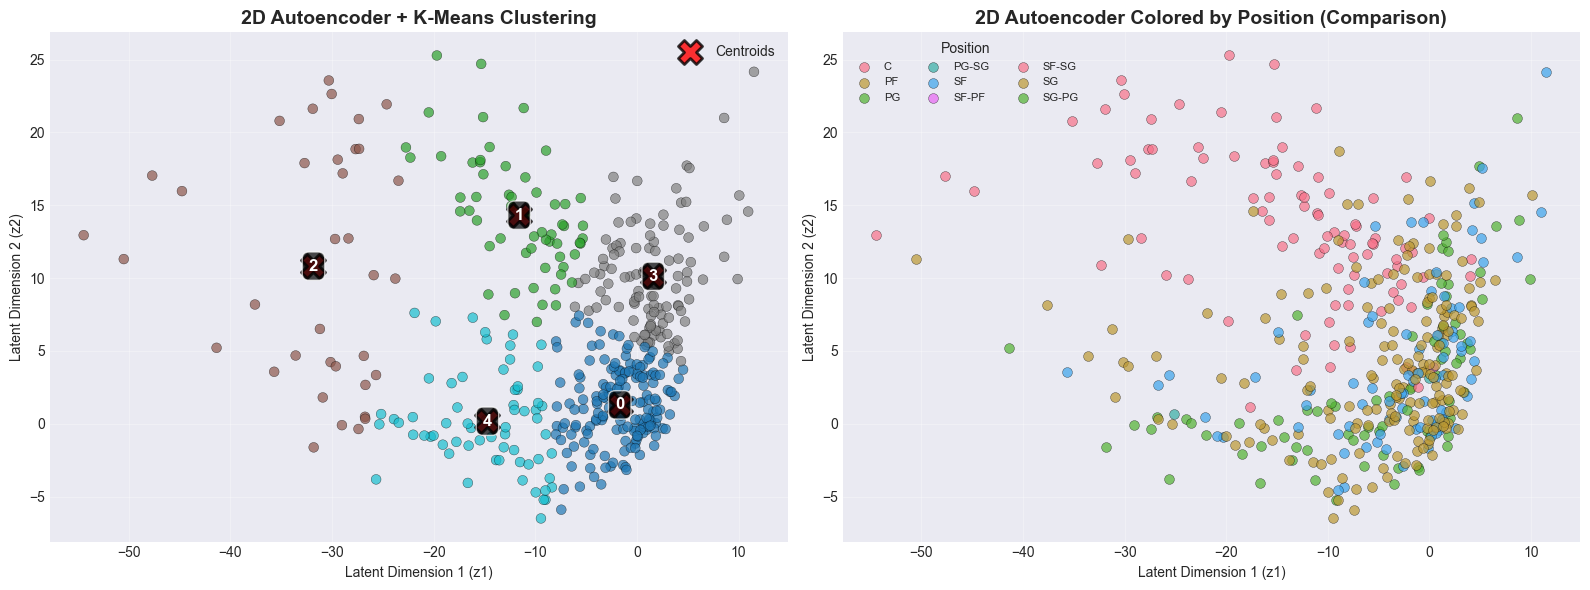
\includegraphics[width=\linewidth]{media/2a.png}
    \caption{Left: 2D Autoencoder latent space with k-Means clusters. Right: Same space colored by traditional positions, showing that statistical similarity transcends positional labels.}
    \label{fig:ae_clustering}
\end{figure}

The clustering reveals five distinct player archetypes: {\bf Cluster 0 (Veteran Role Players)} includes aging stars like John Wall, Klay Thompson, and Khris Middleton with moderate scoring (9.89 PPG) and balanced contributions; {\bf Cluster 1 (Defensive Bigs)} captures rim protectors like Ben Simmons and DeAndre Jordan with low scoring (5.60 PPG) but exceptional rebounding (21.43\% DRB) and shot-blocking (3.85\% BLK); {\bf Cluster 2 (Elite Scoring Guards)} contains the league's premier offensive players including Stephen Curry, Russell Westbrook, and Bradley Beal, averaging 20.02 PPG with elite playmaking (24.08\% AST); {\bf Cluster 3 (Superstar Two-Way Players)} identifies all-around excellence with LeBron James, Kevin Durant, and Giannis Antetokounmpo combining high scoring (17.98 PPG) with superior defensive metrics (23.34\% DRB, 3.52\% BLK); {\bf Cluster 4 (Deep Bench)} consists of players with minimal playing time and production (3.59 PPG) across all categories.

The visualization in Figure~\ref{fig:ae_clustering} demonstrates that the autoencoder learned a meaningful latent space where player impact and playing style are naturally separated. The left side of the latent space contains defensive specialists (Clusters 1 and 3) with high rebounding and blocking, while the center and right contain offensive-focused players (Clusters 0, 2, 4) with varied scoring levels. Comparison with position-based coloring (right panel) reveals that traditional positions fail to capture modern player roles, as statistical similarity transcends positional labels.

\subsection{Autoencoders + Self-organising maps}

\begin{table}[h!]
\centering
\caption{Cluster Statistical Summary (mean values per player group)}
\label{tab:cluster_stats}
\begin{tabular}{lcccccc}
\toprule
\textbf{Cluster} & \textbf{PTS} & \textbf{AST\%} & \textbf{STL\%} & \textbf{BLK\%} & \textbf{ORB\%} & \textbf{DRB\%} \\
\midrule
Blue: Rotational contributors & 8.03 & 13.04 & 1.58 & 1.39 & 3.88 &	12.68 \\
Orange: Defensive players & 6.22 & 10.34 & 1.42 & 2.49 & 7.32 & 16.35 \\
Green: Franchise players & 20.58 & 18.58 & 1.36 & 2.74 & 7.92 & 21.35 \\
Red: Deep Bench & 4.81	& 9.89 &	1.43 &	1.90 &	6.54 &	15.55 \\
Purple: Primary Perimeter Scoring Options & 17.42	&20.77 &	1.43 &	1.39	& 3.60	& 14.81 \\
\bottomrule
\end{tabular}
\end{table}

In this section we made use of the latent vectors derived from the autoencoders in 2.1.a combined with a SOMs approach.
The SOMs approach helps us understand the continuous similarity patterns between the player roles, and we later use it to then derive two graphs: U-matrix and the Player cluster. The U-matrix will be used to show class boundaries:

The {\bf light areas} indicate large distances between the neurons which translates to a strong difference between the group of players.
The {\bf dark areas} indicate small distances between the neurons which are homogeneous regions where players have similar profiles.

Finally we use the Player cluster to help us interpretate the different data points in the clusters and their mapping from the U-matrix gradients. Using SOMs and the averages from the statistical summary table, we see that the player roles are more general and not position specific.

\begin{figure}[h]
    \centering
    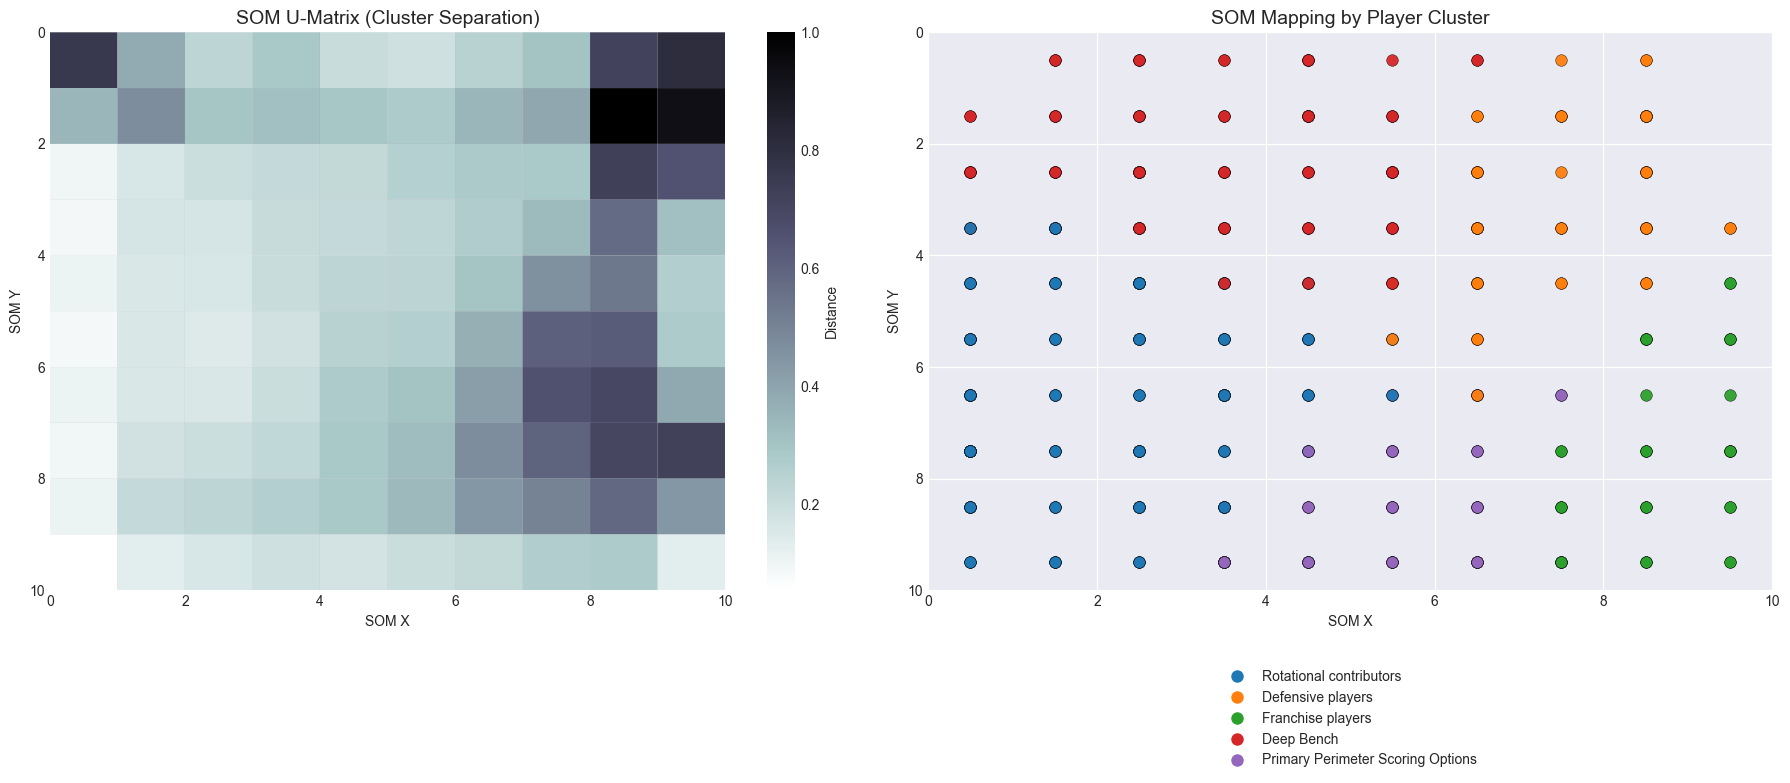
\includegraphics[width=0.7\linewidth]{media/2b.png}
    \caption{SOM U-Matrix showing cluster separation.}
\end{figure}

{\bf Cluster Descriptions:}
\begin{itemize}
    \item \textcolor{blue}{Blue}: Rotational contributors
    \item \textcolor{orange}{Orange}: Defensive players
    \item \textcolor{green}{Green}: Franchise players
    \item \textcolor{red}{Red}: Deep Bench
    \item \textcolor{purple}{Purple}: Primary Perimeter Scoring Options
\end{itemize}

\subsection{Autoencoders + t-SNE}

\begin{table}[h!]
\centering
\caption{Cluster Statistical Summary (mean values per player group)}
\label{tab:cluster_stats}
\begin{tabular}{lcccccc}
\toprule
\textbf{Cluster} & \textbf{PTS} & \textbf{AST\%} & \textbf{STL\%} & \textbf{BLK\%} & \textbf{ORB\%} & \textbf{DRB\%} \\
\midrule
0: Bench role players & 6.98 & 12.19 & 1.52 & 1.47 & 4.00 & 12.83 \\
1: Defensive players & 6.19 & 10.43 & 1.43 & 2.24 & 6.81 & 16.60 \\
2: Secondary playmakers & 13.08 & 16.68 & 1.57 & 1.31 & 3.30 & 12.97 \\
3: Players with limited minutes & 4.93 & 10.13 & 1.44 & 1.92 & 6.65 & 15.37 \\
4: Primary scoring starters & 20.04 & 20.76 & 1.42 & 2.12 & 6.13 & 18.30 \\
\bottomrule
\end{tabular}
\end{table}

This section uses the t-SNE approach which helps us focus on local similarity, preserving players who are close in feature space and it is also useful for visualizing distinct roles clearly. For our interpretation we will make use of the cluster statistical summary and the K-Means clustering.

By using the table of averages above is how we were able to properly describe the clusters:

{\bf Cluster 0:} Bench role players with a moderate average of assists as well as defensive rebounds. Meaning, the players in this cluster are good on defense and they can set up the plays, but lack in scoring stats.

{\bf Cluster 1:} Defensive players. These players tend to be quite tall compared to the others which facilitates in ball possession, and this is backed up by the offensive/defensive rebound averages, however even though they can get a moderate average of assists, their scoring ability is a weakness.

{\bf Cluster 2:} Secondary playmakers also called the 6th man. These players are in charge of setting up the plays, while also being able to score themselves and participate on the defence. They are players who ensure good ball movement on the court, and we see this by looking at the points, average of assists and defensive rebound. 

{\bf Cluster 3:} Players with limited minutes. In the basketball roster the role and talent of a player speaks volumes, and often we get players who are not able to perform at the high level or given opportunities in a team full of talents. Most of these players are quite good on defence and assists, but lack heavily on the scoring sheet.

{\bf Cluster 4:} Starters. These players are all-rounders when it comes to playmaking, scoring and defensive abilities and they compose the 5 main players of the roster.

\begin{figure}[h]
    \centering
    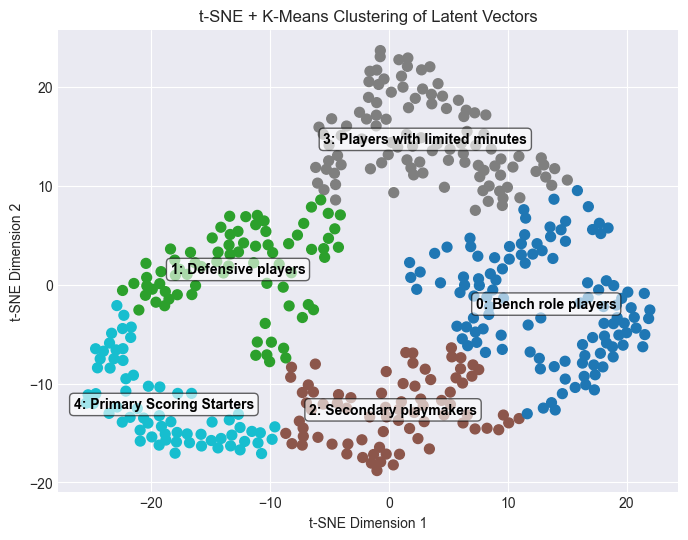
\includegraphics[width=0.7\linewidth]{media/2c.png}
    \caption{t-SNE + K-Means Clustering.}
\end{figure}

\subsection{Autoencoders + UMAP}

UMAP (Uniform Manifold Approximation and Projection) provides an alternative dimensionality reduction approach that preserves both local and global structure of the data. We applied UMAP to the 2D autoencoder latent vectors with parameters: 20 neighbors, minimum distance of 0.1, and random initialization (random seed 42). Unlike t-SNE which focuses primarily on local similarity, UMAP better preserves the global structure while maintaining computational efficiency and producing more stable embeddings.

Following UMAP dimensionality reduction, we applied k-Means clustering (k=5) to identify player archetypes. Table~\ref{tab:umap_cluster_stats} presents the statistical profiles of the discovered clusters.

\begin{table}[h!]
\centering
\caption{UMAP K-Means Cluster Statistical Summary}
\label{tab:umap_cluster_stats}
\begin{tabular}{lcccccc}
\toprule
\textbf{Cluster} & \textbf{PTS} & \textbf{AST\%} & \textbf{STL\%} & \textbf{BLK\%} & \textbf{ORB\%} & \textbf{DRB\%} \\
\midrule
0: 3\&D Wings & 7.47 & 12.43 & 1.50 & 1.40 & 3.53 & 12.42 \\
1: Bench Specialists & 9.09 & 13.39 & 1.61 & 1.67 & 4.50 & 13.93 \\
2: Star Scorers/Bigs & 5.00 & 9.79 & 1.39 & 1.97 & 6.29 & 14.71 \\
3: Limited-Min Starters & 5.37 & 10.73 & 1.47 & 1.68 & 6.03 & 14.97 \\
4: Lead Guards & 14.91 & 17.23 & 1.40 & 2.07 & 6.15 & 17.21 \\
\bottomrule
\end{tabular}
\end{table}

The UMAP clustering reveals five distinct player groups with more granular role definitions compared to the autoencoder-only approach: {\bf Cluster 0 (3\&D Wings)} captures role players like Nicolas Batum, Eric Gordon, and Joe Harris who specialize in three-point shooting and defense with moderate scoring (7.47 PPG); {\bf Cluster 1 (Bench Specialists)} includes veteran contributors like John Wall, Klay Thompson, and Khris Middleton with balanced production (9.09 PPG, 13.39\% AST); {\bf Cluster 2 (Star Scorers/Bigs)} identifies emerging talent and role bigs like Nerlens Noel and Keldon Johnson with lower scoring (5.00 PPG) but solid rebounding presence (6.29\% ORB); {\bf Cluster 3 (Limited-Minute Starters)} contains players like Kemba Walker and Evan Fournier transitioning to reduced roles (5.37 PPG); {\bf Cluster 4 (Lead Guards)} captures the league's elite including Stephen Curry, LeBron James, Kevin Durant, and Russell Westbrook with the highest scoring (14.91 PPG) and playmaking (17.23\% AST).

\begin{figure}[h]
    \centering
    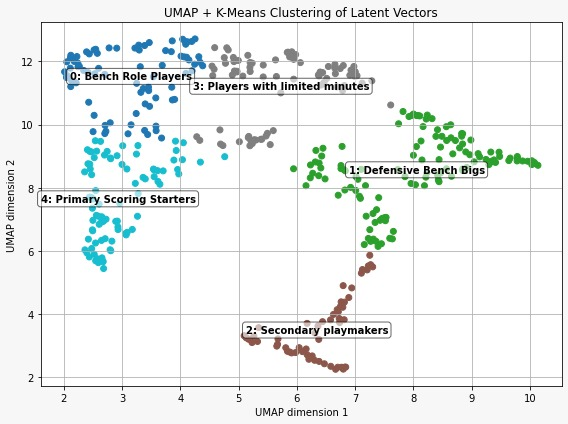
\includegraphics[width=0.7\linewidth]{media/2d.png}
    \caption{UMAP + K-Means Clustering showing preserved global structure with distinct player archetypes.}
    \label{fig:umap_clustering}
\end{figure}

The UMAP visualization in Figure~\ref{fig:umap_clustering} demonstrates clearer cluster separation compared to t-SNE, with the elite players (Cluster 4) forming a distinct region, while role players and specialists occupy separate but connected regions. The preservation of global structure allows for better interpretation of the relationships between different player archetypes, showing how bench specialists (Cluster 1) transition into elite roles (Cluster 4), while 3\&D wings (Cluster 0) and limited-minute players (Cluster 3) occupy more specialized niches in the player ecosystem.

\end{document}
